\documentclass{article}

\usepackage{ftdstyle}
\usepackage{times}
\usepackage{stfloats}
\usepackage{indentfirst}
\usepackage{caption}
\usepackage{subcaption}

\usepackage{graphicx}
\graphicspath{{images}}

\usepackage[hyphens]{url}
\usepackage[colorlinks=true, linkcolor=, urlcolor=blue, citecolor=]{hyperref}
\hypersetup{
	pdfauthor="Aleksandr Sergeev",
	pdftitle="Comparison of neural network and algorithmic based person detectors for LiDAR data"
}

\title{
    Comparison of neural network and algorithmic based person detectors for LiDAR data
}

\author{
    Aleksandr Sergeev \\ 
    Grenoble, France \\
    \href{mailto:aleksandr.sergeev@etu.univ-grenoble-alpes.fr}{\textcolor{black}{aleksandr.sergeev@etu.univ-grenoble-alpes.fr}} \\
    \\
    Supervised by: Olivier Aycard
}

\begin{document}

\maketitle{
    \hbox to0pt{
        \vbox{
            \baselineskip=10dd
            \hrule
            \hbox to\hsize{
                \kern-3pt
                \vrule
                \vbox{
                    \kern3pt
                    \hbox{
                        \small I understand what plagiarism entails and I declare that this report
                    }
                    \hbox{
                        \small is my own, original work.
                    }
                    \hbox{
                        \small Name, date and signature: Aleksandr Sergeev, 21.09.2023.
                    }
                }
                \hfil
                \vrule
            }
            \hrule
        }
    }
}

\parbox[b]{\linewidth}{}

\begin{abstract}
	This paper looks at two different ways to find people using information from 2D LiDARs, and it checks how well they work.
	One method is called the "algorithmic detector".
	It uses a clever way to find people by looking for groups of points that are close together.

	The other method is called the "DROW detector".
	It uses a computer program that's like a brain (a neural network).
	This brain learned from the latest DROW dataset and uses information from the five most recent LiDAR scans to guess where people are, thinking about how things change over time.

	To see how good these detectors are, the scientists tested them using live data and also data from the DROW dataset.
	They made a special "\texttt{follow\_the\_drow}" library, a Robot Operating System (ROS) package, and a Docker image to help compare and use the detectors.

	When they compared the two detectors, they saw that the DROW detector is more accurate with the DROW dataset.
	But, they noticed some mistakes in how the data was marked, so they aren't completely sure about the results.

	In the end, even though the algorithmic detector did better in the lab, detectors that learn from good data have more potential in the real world.
	The scientists suggest that future work should try to make the neural network work faster and make sure the data is marked correctly.
\end{abstract}

\section{Introduction}

LiDAR technology is used in many areas\cite{lidar_market}.
While 3D LiDARs are becoming more common, 2D LiDARs are still used in robots\cite{lidar_popularity} and self-driving cars\cite{lidar_autonomous}.
Finding people with LiDAR is hard because people are important to identify, especially in self-driving cars. 
eople can look different in 2D pictures.

This study compares two ways to find people.
One uses a special method to find where people are.
It looks for groups of points close to each other and thinks of them as "legs".
If it sees two "legs" close together, it says it found a "person".
We'll call this the "algorithmic detector".

The other way uses a computer program called a neural network, which learned from data in the "Deep Person Detection in 2D Range Data" article\cite{DROW_2018} and uses data from that article's GitHub.
This computer program uses special layers to process data.
It looks at the five most recent measurements from LiDAR to guess where people are.
We'll call this the "DROW detector" because that's what it's called in the article.

The robots that use these detectors, Karl for the DROW detector and RobAIR for the algorithmic detector\cite{RobAIR_site}, are very similar.
They both use 2D LiDAR with the same view angle.
They put the LiDAR at the same height.
This means we could use the same data to test and compare both ways to find people.

\section{Comparison of person detectors}

\begin{figure*}[t!]
	\centering
	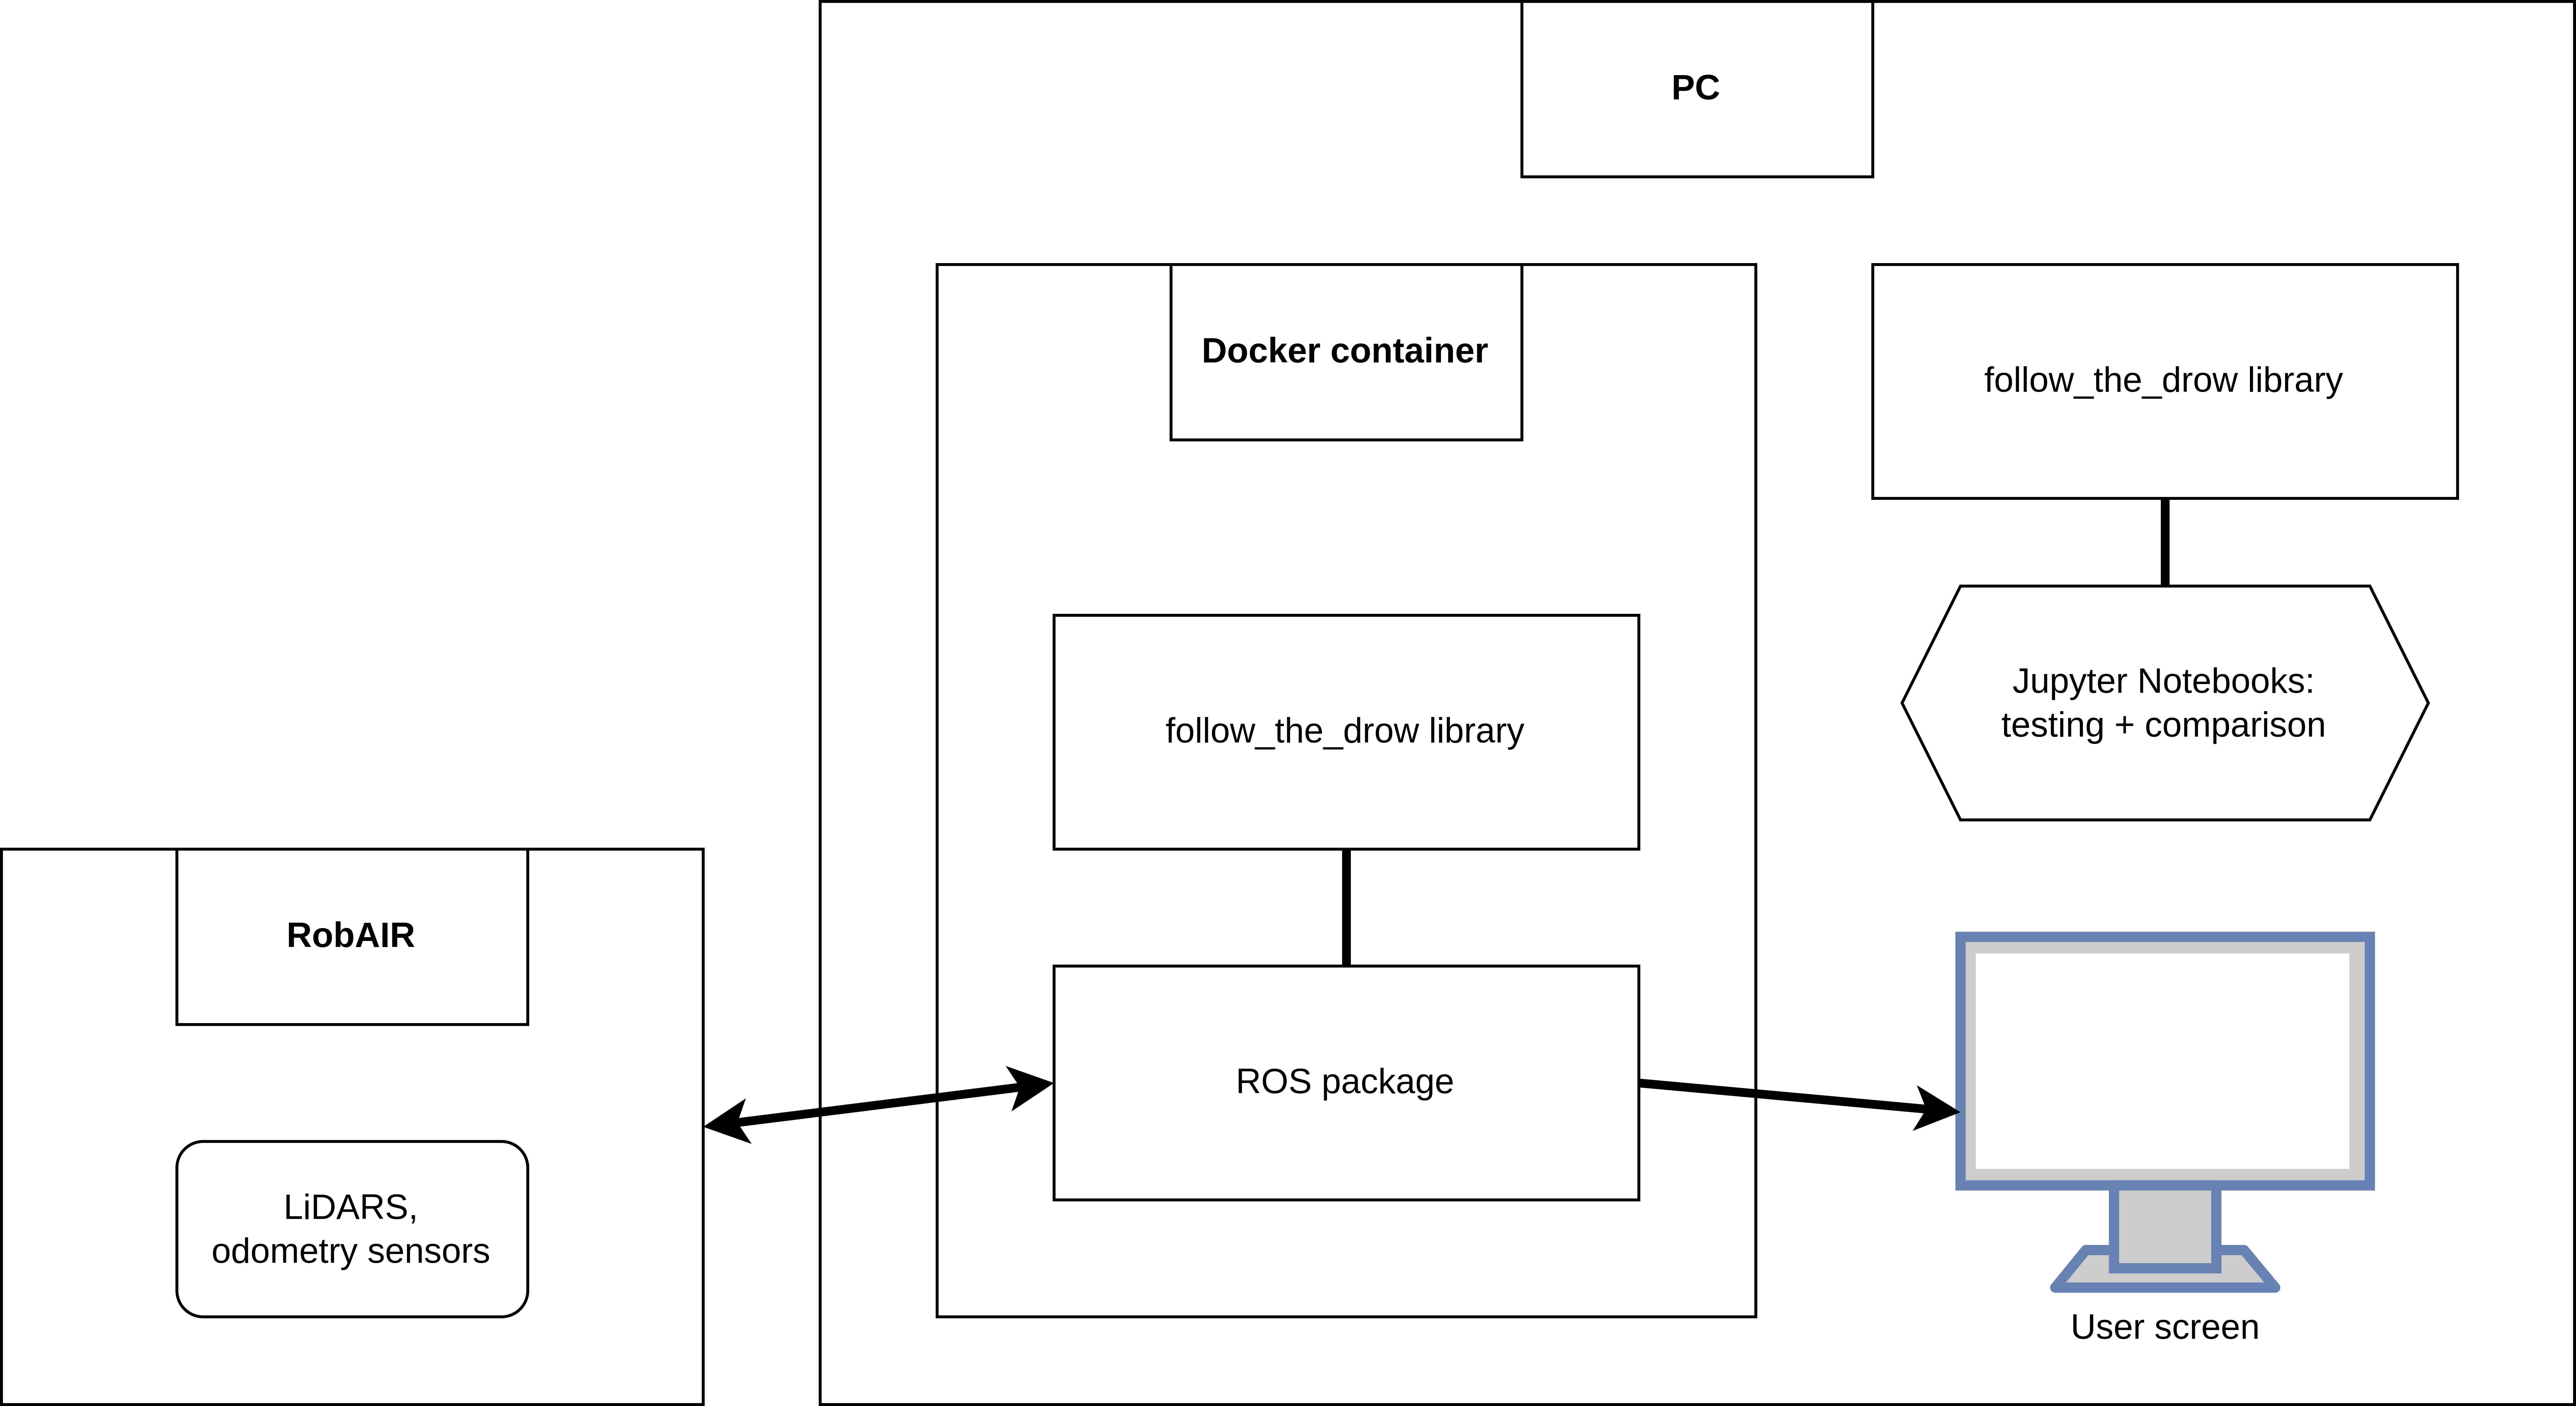
\includegraphics[width=0.9\textwidth]{ftd_setup_chart}
	\caption{Library and package setup chart}
	\label{fig:ftd_setup_chart}
\end{figure*}

To compare the algorithmic and DROW detectors, we needed to make them work in the same places and use the same data.
We made a special library to use both detectors with a computer program called \texttt{Python}.

For using the detectors on RobAIR, we made a package for something called the Robot Operating System (ROS)\cite{ros_site}.
It helps robots work better.
This package has parts that help collect LiDAR data, change it, and make the detectors work.
We also made something called Docker, which is like a special box for the computer code
It lets you run the detectors on computers that don't have ROS.

In Figure \ref{fig:ftd_setup_chart}, you can see how we set everything up to make the detectors work and compare them.
We compared them on a regular computer using the DROW dataset and a thing we made called \texttt{follow\_the\_drow} library.
We wrote down the results in special notebooks.
We also tested the detectors in real-time on a regular computer connected to RobAIR.
We used the \texttt{follow\_the\_drow} ROS package inside a Docker box.
It got the live data from RobAIR's sensors and showed the results on the computer screen with a thing called RVIZ\cite{rviz_wiki}.

The \texttt{follow\_the\_drow} library, the ROS package, and the Docker box are things we made for this project.
You can use them to compare different detectors and run computer programs, even if you don't have a real robot.
You might need to make some small changes, but they should be helpful.

\subsection{\texttt{follow\_the\_drow} library}

The library has three main parts.

The first part is called "Datasets".
It has the dataset from the DROW article, and it comes with some helpful ways to load and get data from it.
There's also another dataset called the "live dataset" that's useful for working with data that comes from robot scanners while they are working.

The second part is the "Detector" part.
It has the DROW detector, which can find where people are.
It also has some methods that make it easier to work with the votes that show where the detector thinks people are.
Additionally, there's a \texttt{Python} wrapper for the algorithmic detector.
Originally, the algorithmic detector was written in \texttt{C++}, and the \texttt{C++} code is also in the library.

The last part is "Utilities".
This part has functions that the authors of the DROW article used in their public repository.
It also includes some other helpful methods for automatically getting the DROW dataset and saving the results.

\subsubsection{DROW dataset provider}


The DROW dataset comes with the \texttt{follow\_the\_drow} library, and you don't need to get it separately.
The dataset provider loads all the data into memory at once. 
This dataset has information from just one LiDAR, which is placed at knee height.
Because of this, there is only one way to get the data, and it's called the "bottom" data.

The DROW detector looks at the five most recent measures, but the algorithmic detector looks at one detection at a time.
So, the retrieval function combines one or more of the most recent measures into an array to make it work together.

\subsubsection{Live dataset provider}

The live dataset provider pretends to be a dataset for real-time data.
It collects measurements in a line of things that are asked for, and when you want the data, it gives it to you and clears the line.
It can also handle getting data from two LiDARs at the same time and providing it to the detector when needed.

\subsubsection{DROW person detector}

The DROW person detector is based on the DROW article\cite{DROW_2018}.
It uses a neural network model created with the pytorch\cite{pytorch_site} library.
This neural network gives its opinion on where objects might be found in a window around each measurement point.
It checks the most recent five measurements to keep track of how the input data changes over time.
However, it can only work with measurements from the bottom LiDAR.

The detector provides arrays of votes and confidences.
These can be changed into predictions about where people might be found using the library's functions.

\subsubsection{Algorithmic person detector}

The algorithmic person detector is based on the \textbf{Follow me behavior} article\cite{follow_me_behavior}.
It was modified to use advanced \texttt{C++} features like links and vectors and can be changed while it's running.
This algorithm looks for objects that show specific patterns of "clusters" of points that are very close to each other.
It can work with measurements from the bottom LiDAR (15cm from the ground), the top LiDAR (1.6m from the ground), or both together.
The detector provides an array of positions where it thinks people might be.

The Follow the DROW library also includes a connection between the algorithm's \texttt{C++} code and a \texttt{Python} class using the texttt{pybind11}\cite{pybind_site} library.
This makes it possible to use the algorithm in Python.

\subsection{Follow the DROW ROS package}

\begin{figure*}[t!]
	\centering
	\includegraphics[width=0.9\textwidth]{ftd_package_chart}
	\caption{Follow the DROW ROS package chart}
	\label{fig:ftd_package_chart}
\end{figure*}

\begin{figure}[b!]
	\centering
	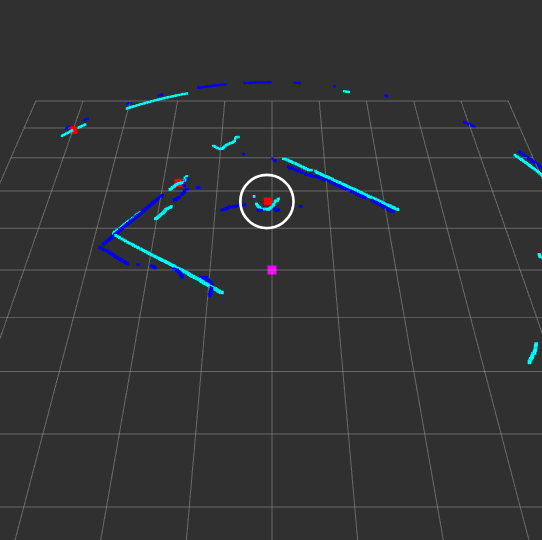
\includegraphics[width=0.75\linewidth]{ftd_live_output}
	\caption{Visualizer node live output}
	\label{fig:visualizer_node_live}
\end{figure}

We made a special ROS package for running the detectors on a regular computer and using data from the real world (RobAIR).
To use this package, you need the \texttt{follow\_the\_drow} library.

In Figure \ref{fig:ftd_package_chart}, you can see a picture that shows the different parts of the follow the DROW ROS package and how they read data from and write data to different places.
The package has these parts:

\begin{enumerate}
	\item \textbf{Live Loader} takes data from RobAIR's LiDAR(s), and you can choose which topics to use for input. Then, it gives you the measurements from the LiDAR and data about how RobAIR is moving, which is called odometry data.
	\item \textbf{File Loader} gets data from the DROW dataset, and then it gives you the measurements from the dataset and information about how the robot is moving, which is called odometry data.
	\item \textbf{Algorithmic detector} uses the algorithmic detector to work with the data, and the result is an array of positions where it thinks people might be.
	\item \textbf{DROW detector} uses the DROW detector to analyze the data, and the result is an array of positions where it thinks people might be.
	\item \textbf{Person tracker} follows one person from the arrays that are given by the chosen detector node. There are different ways it can do this, which are called tracking policies.
	\item \textbf{Visualizer} shows all the data in the system, which includes the raw measurements, information about what's in the data, where it thinks things are (detections), and where it believes a person is being tracked.
	\item \textbf{Annotator} can help with changing the annotations in the DROW dataset manually. It uses the RVIZ interface to let you adjust where it thinks a person is located.
\end{enumerate}

We tell the robot, RobAIR, some details about itself.
We say that the middle part of RobAIR is right in the middle at the bottom.
We also say that one of its LiDARs is 15cm in front, and the other is 1.2 meters above.

In the figure \ref{fig:visualizer_node_live}, you can see what the robot is seeing.
The robot is shown in pink.
There are dark blue dots for the bottom LiDAR, light blue dots for the top LiDAR, and red dots show where the robot thinks people are.

There should be green dots for where another way of finding people, called DROW, thinks people are, but it didn't find anyone.
The white circle shows where the robot is sure there's a person, but the other predictions are not right.

\subsection{Follow the DROW Docker image}

\begin{figure*}[t!]
	\centering
	\begin{subfigure}{.5\textwidth}
		\centering
		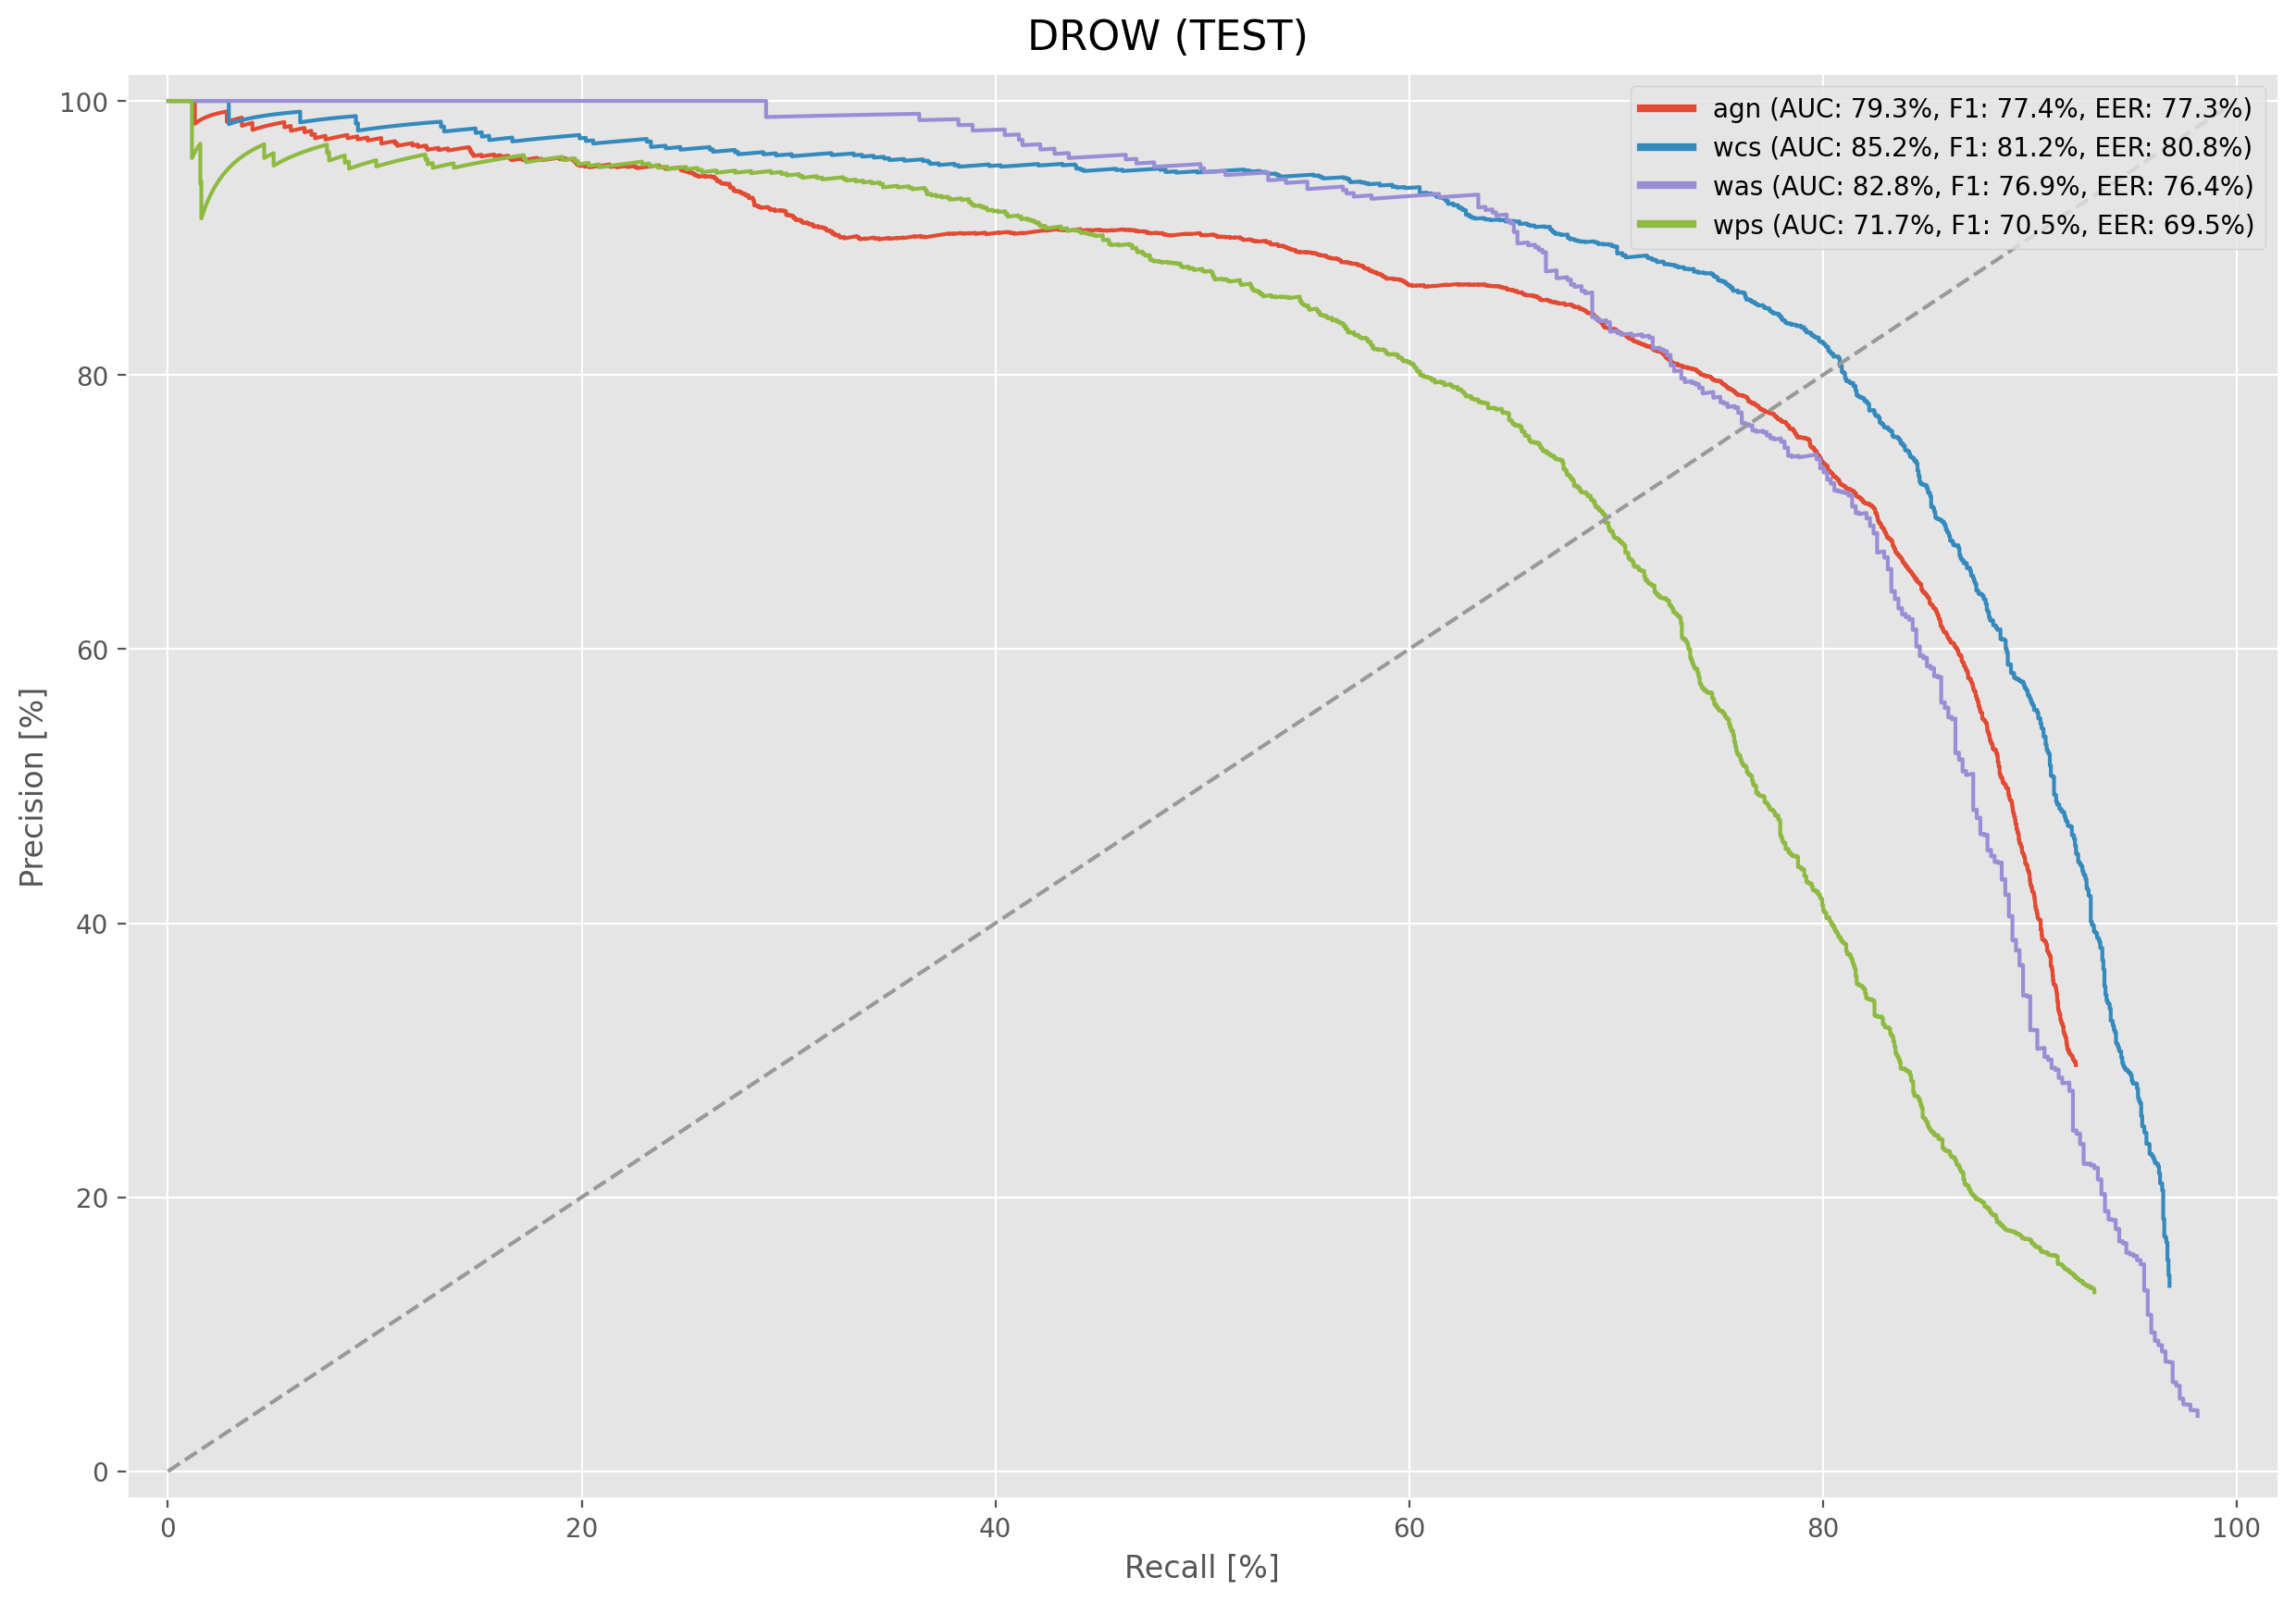
\includegraphics[width=.9\linewidth]{pr_auc_drow}
		\caption{Precision-recall curve of DROW detector}
		\label{fig:pr_auc_drow}
	\end{subfigure}%
	\begin{subfigure}{.5\textwidth}
		\centering
		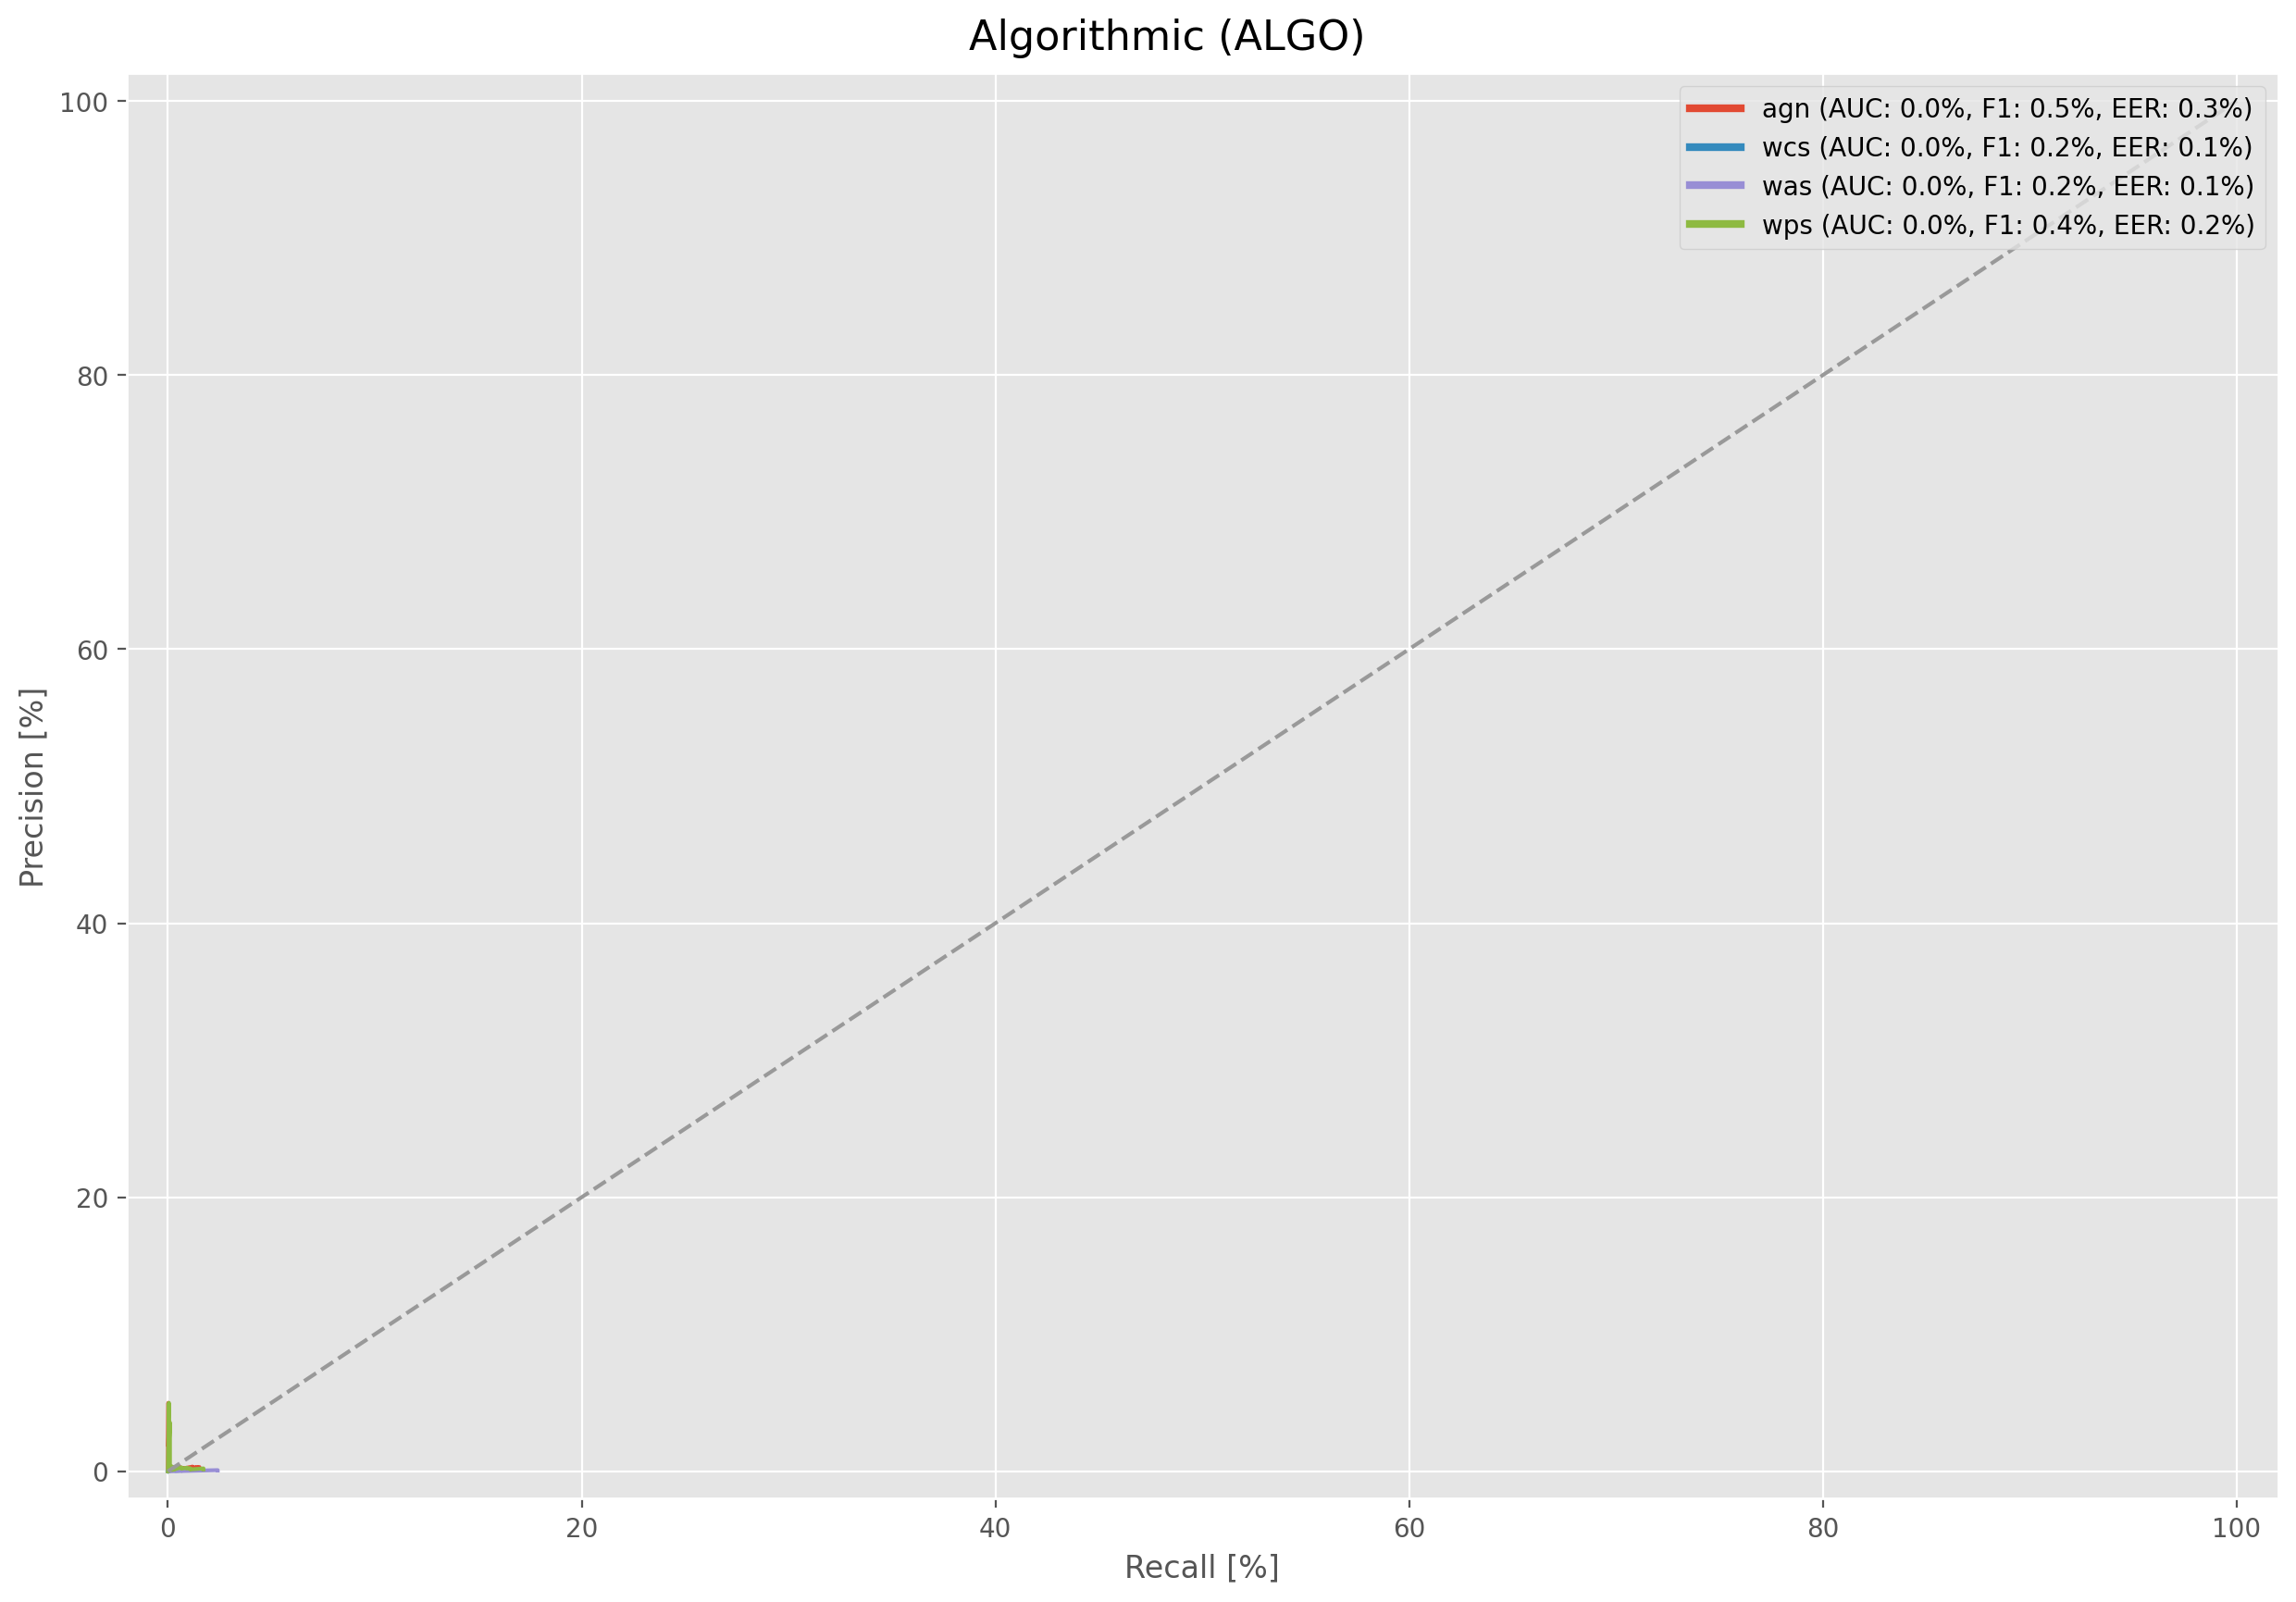
\includegraphics[width=.9\linewidth]{pr_auc_algo}
		\caption{Precision-recall curve of algorithmic detector}
		\label{fig:pr_auc_algo}
	\end{subfigure}
	\caption{Comparison of detectors precision-recall curves}
	\label{fig:pr_auc_comparison}
\end{figure*}

To use the latest ROS 1, which only works on Ubuntu Focal Fossa (20.04), we made a special Docker image.
First, we created an image with the complete ROS system.
It has all the ROS parts, a workspace called \texttt{catkin}\cite{catkin_wiki}, and a script to set things up.
You can find this image on GitHub\cite{FTD_docker_image}.

Then, we made another image that includes the \texttt{follow\_the\_drow} library.
It's a big file, so we can't share it, but you can build it on your own computer.

We also made a Docker setup that takes care of things like showing pictures with RVIZ.
It's set up to work with RobAIR if you want.

\section{Results}

We compared the detectors on a laptop using data from the DROW dataset.
To save and look at the results, we used Jupyter notebooks.
You can see these notebooks in the paper's GitHub repository\cite{FTD_comparison}.

\subsection{Precision-recall comparison}

\begin{figure*}[t]
	\centering
	\begin{subfigure}{.5\textwidth}
		\centering
		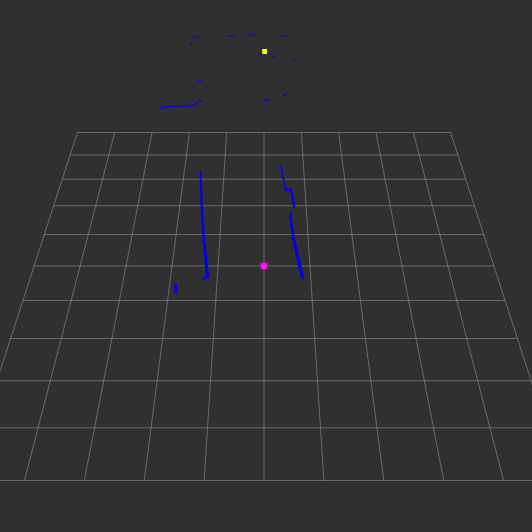
\includegraphics[width=.65\linewidth, height=.65\linewidth]{ftd_false_negative_1}
		\caption{}
		\label{fig:drow_false_negative_1}
	\end{subfigure}%
	\begin{subfigure}{.5\textwidth}
		\centering
		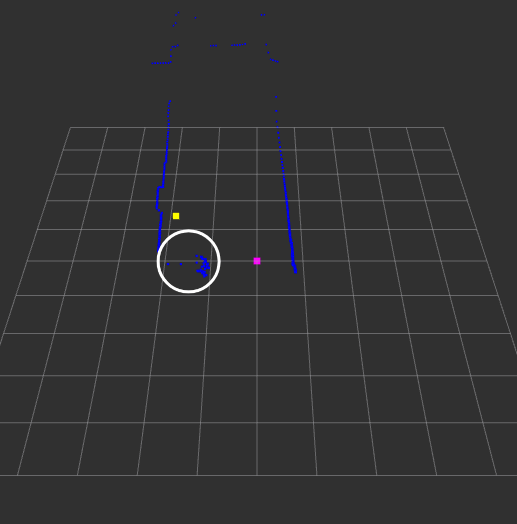
\includegraphics[width=.65\linewidth, height=.65\linewidth]{ftd_false_negative_2}
		\caption{}
		\label{fig:drow_false_negative_2}
	\end{subfigure}
	\parbox[b]{\textwidth}{}
	\begin{subfigure}{.5\textwidth}
		\centering
		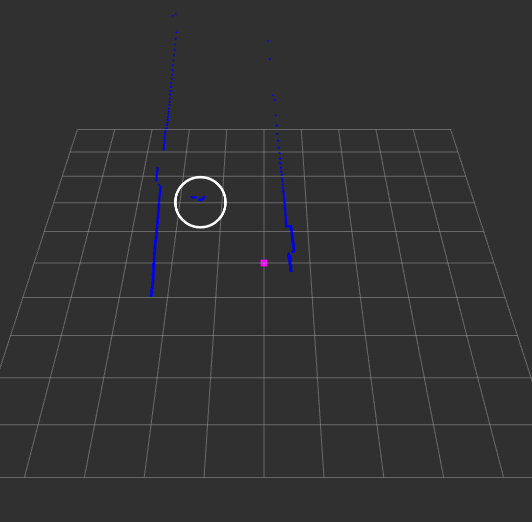
\includegraphics[width=.65\linewidth, height=.65\linewidth]{ftd_false_positive_1}
		\caption{}
		\label{fig:drow_false_positive_1}
	\end{subfigure}%
	\begin{subfigure}{.5\linewidth}
		\centering
		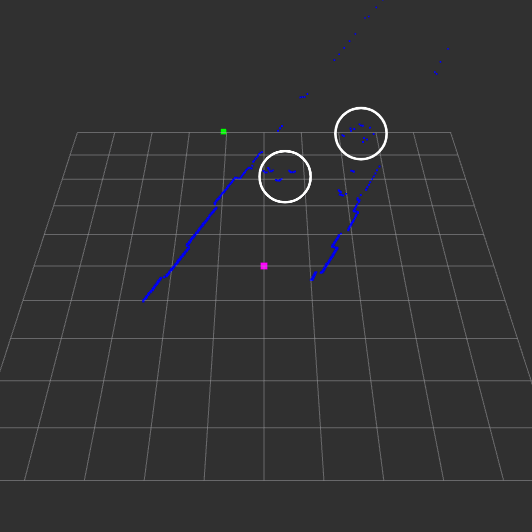
\includegraphics[width=.65\linewidth, height=.65\linewidth]{ftd_false_positive_2}
		\caption{}
		\label{fig:drow_false_positive_2}
	\end{subfigure}
	\caption{DROW dataset incorrect annotation examples}
	\label{fig:drow_annotation_errors}
\end{figure*}

We compared how well the detectors work by looking at something called the AUC of the precision-recall curve.
This helps us see how accurate the detectors are.
In Figure \ref{fig:pr_auc_comparison}, you can see some lines that show how good the detectors are.
We used the DROW dataset to see where people really are.

In the picture, the green dots are where the DROW detector thinks people are, and the yellow dots are where the DROW dataset says people are.
The pink dot is the robot.
There were some problems with the yellow dots because they didn't match where the people really were.
Some people were missed (Figures \ref{fig:drow_false_negative_1} and \ref{fig:drow_false_negative_2}), and some were wrongly marked (Figures \ref{fig:drow_false_positive_1} and \ref{fig:drow_false_positive_2}).
We found out that the yellow dots were only right for about 20 seconds in the first 3 minutes of the DROW dataset.

Because of these problems, the neural network trained on this data can't find people very well.

\subsection{Execution time comparison}


We compared how fast the detectors work by measuring how much time each detector needs to process one LiDAR measurement.
Here are the results:

\begin{itemize}
	\item \textbf{DROW detector} 0.9771 seconds.
	\item \textbf{Algorithmic detector} 0.0001 seconds.
\end{itemize}

RobAIR doesn't have a special graphics chip, so we decided to run tests on a computer without one, too.
The computer has an Intel\textregistered{} Core\texttrademark{} i7-3520M CPU running at 2.90GHz, and it has its own built-in graphics.

Even though we set the test to run at 10 times per second, which is faster than when we recorded the DROW dataset (that was 12.5 times per second), it wasn't enough to run the DROW detector every time.
But this didn't make the other parts work slower because they run in their own separate places.
The only thing you might notice is that the DROW detector markers are updated only once per second.

\section{Conclusion and future work}

People often choose 2D LiDARs because they're cheaper and don't need as much computer power as 3D LiDARs and cameras\cite{2D_3D_lidars}.
This is important for self-driving vehicles.

In this paper, we looked at two ways to find people: one uses a guessing method, and the other uses a smart computer system inspired by VGGnet\cite{vggnet_paper}.
We tried both methods with the DROW dataset, but the results are not really helpful because the dataset has wrong information.
In the real world, the guessing method works better sometimes, but this doesn't mean the smart computer method is bad.
It just depends on the information used to train it.
And the guessing method can't find some things, like wheelchairs or people in lab coats.

We also made a system called \texttt{follow\_the\_drow} to use these methods and test them.
Here's what it can do:
\begin{itemize}
	\item library in \texttt{Python} for testing detectors that also has connections to \texttt{C++} code.
    \item tool in ROS to set up and compare detectors that works with the \textbf{Follow me behavior} packages.
	\item image for Docker that helps run the latest ROS 1 system on any Linux device, including the \texttt{follow\_the\_drow} package. You can use it on your computer or a real robot.
\end{itemize}

Please check the paper's README file\cite{FTD_repo_readme} for info on setting up the ROS package and using commands to test and compare detectors.
You can also look at the Docker image README\cite{FTD_image_readme} for info on how to use and customize it for other ROS packages.

To fix the issue with incorrect annotations, we made an \texttt{Annotator} tool that lets you change the dataset manually using a graphical interface in RVIZ.
To make the neural network work faster, we can think about these steps in the future:
\begin{enumerate}
	\item The \texttt{pytorch} library works with both \texttt{Python} and \texttt{C++}, which can make the network run faster.
    \item To make the network work better, we can use a design with recurring layers instead of processing 5 LiDAR measures together. This can also make the network more accurate, as explained in the latest DROW article\cite{DROW_2018}.
	\item Using only the most recent LiDAR measurement doesn't just make calculations faster but also helps use odometry data better. For example, instead of doing math again, we can just give the network the difference between odometry data in frames.
\end{enumerate}

In a lab, the algorithmic detector was quicker and better.
But for real life, where we need to handle specific cases it can't, a DROW or similar neural network-based detector trained with good data is a better choice.

\clearpage

\bibliographystyle{named}
\bibliography{ftdbibl}

\end{document}
